
\documentclass[10pt,twocolumn,a4paper]{article}

% ============================================================
% PACKAGES
% ============================================================

% Typography and layout
\usepackage[T1]{fontenc}
\usepackage[utf8]{inputenc}
\usepackage{lmodern}
\usepackage{microtype}
\usepackage{xcolor}
\usepackage[margin=0.75in,columnsep=0.25in]{geometry}

% Mathematics
\usepackage{amsmath}
\usepackage{amssymb}
\usepackage{amsfonts}
\usepackage{amsthm}
\usepackage{bm}
\usepackage{mathtools}

% Figures and tables
\usepackage{graphicx}
\usepackage{subcaption}
\usepackage{booktabs}
\usepackage{multirow}
\usepackage{float}

% Algorithms
\usepackage{algorithm}
\usepackage{algpseudocode}

% References and links
\usepackage[numbers,sort&compress]{natbib}
\usepackage[
    colorlinks=true,
    linkcolor=blue!50!black,
    citecolor=blue!50!black,
    urlcolor=blue!50!black
]{hyperref}


% Miscellaneous
\usepackage{enumitem}
\usepackage{balance}

\raggedbottom  % do not stretch paragraph spacing to fill columns

% ============================================================
% CUSTOM COMMANDS
% ============================================================

\newcommand{\R}{\mathbb{R}}
\newcommand{\N}{\mathbb{N}}
\newcommand{\vect}[1]{\bm{#1}}
\newcommand{\mat}[1]{\bm{#1}}
\newcommand{\loss}{\mathcal{L}}
\newcommand{\data}{\mathcal{D}}
\newcommand{\E}{\mathbb{E}}
\newcommand{\norm}[1]{\left\lVert#1\right\rVert}
\newcommand{\sh}[2]{\ensuremath{#1{\times}#2}}  % model shape: width x depth

\DeclareMathOperator*{\argmin}{arg\,min}
\DeclareMathOperator*{\argmax}{arg\,max}

\newtheorem{theorem}{Theorem}
\newtheorem{proposition}{Proposition}
\newtheorem{lemma}{Lemma}
\newtheorem{definition}{Definition}





% ============================================================
% TITLE AND AUTHORS
% ============================================================

\title{\textbf{Experiments on width-depth ratios, parameterisations, and learning rate schedules for LLM training}}

\author{
    Caio Artus\\
    \small Student ID : A0350346J\\
    \small Group number : 9\\
    \small \texttt{caio.artus@u.nus.edu}\\
    \small Code: \href{https://github.com/caioartus/LLM-depth/tree/llm-depth}{\texttt{github.com/caioartus/LLM-depth/tree/llm-depth}}
}

\date{}

% ============================================================
% DOCUMENT
% ============================================================

\begin{document}

\twocolumn[
\maketitle

\begin{abstract}
We investigate how model width, depth, and parameterisation affect language model performance under a fixed compute budget. We train five Transformer shapes of approximately 50M non-embedding parameters under the standard parameterisation (SP) and CompleteP, comparing a learning rate tuned on one shape and transferred to the others with learning rates tuned per shape. We find that excessively deep models underperform under both parameterisations. CompleteP reduces the loss penalty of transferring the learning rate to the deepest shape, although its absolute loss is slightly higher than SP's at the shapes where both perform best. Unexpectedly, learning rates tuned per shape sometimes perform worse than transferred ones. We trace this to short tuning runs whose compressed schedule leaves a very short warmup, which biases tuning towards low learning rates.
\end{abstract}

\vspace{0.5cm}
]

% ============================================================
\section{Introduction}
% ============================================================


Choosing the dimensions of a Transformer \citep{vaswani2017attention} language model is still an open problem. Scaling laws tell us how to split a compute budget between parameters and training tokens \citep{kaplan2020scaling,hoffmann2022training}, but they say little about how to spend those parameters: on width or on depth. We are interested in the aspect ratio (the width-to-depth ratio $d/L$) that makes a model train efficiently and perform well under a fixed compute budget.

The common view is that width should be scaled faster than depth, and that deep and narrow models are harder to train. \citet{kaplan2020scaling} report that a wide range of shapes perform similarly at a fixed parameter count. \citet{levine2020limits} argue that depth only helps up to a threshold that grows logarithmically with width. \citet{mcleish2025gemstones_v1} fit scaling laws over width and depth and initially concluded that it is better to err towards wider, shallower models; their final version \citep{mcleish2025gemstones} instead finds deeper models better per FLOP, with wider ones ahead only in wall-clock time. More recently, \citet{fahim2026depth} go further and claim that past a critical depth, adding layers increases the loss even though it adds parameters, an effect they call the \emph{Depth Delusion}.

A separate line of work studies parameterisation: the rules for scaling initialisation, learning rates and multipliers with model size. Under SP, the optimal learning rate drifts when the model shape changes. The maximal update parameterisation ($\mu$P) \citep{yang2021feature,yang2022tensor} fixes this for width: hyperparameters can be tuned on a narrow model and transferred to a wider one. Depth-$\mu$P \citep{yang2024depth} and \citet{bordelon2024depthwise} extend the idea to depth by scaling each residual branch by $L^{-1/2}$. CompleteP \citep{dey2025completep} scales it by $L^{-1}$ instead, and shows it is the unique choice that gives both depth-wise learning rate transfer and non-lazy feature learning. They also show that under CompleteP a broader range of aspect ratios stays close to compute-optimal.

This raises our question: did the critics of deep models take parameterisation into account? Mostly not. \citet{fahim2026depth} train every shape under SP with a single learning rate that is never retuned for the deeper models. \citet{dey2025completep} make the same remark about earlier studies: \citet{kaplan2020scaling} use SP, and the learning rate scaling in the first version of \citet{mcleish2025gemstones_v1} does not transfer across depth, which put their deeper models at a disadvantage. A deep model trained with a learning rate tuned for a shallower one is a detuned model, and its loss says as much about the tuning as about the depth. So how much of the depth penalty comes from depth itself, and how much from a poor parameterisation or a detuned learning rate?

To answer this, we train five models of roughly 50M non-embedding parameters with $d/L$ ranging from 4 to 256, all at the same FLOP budget, under both SP and CompleteP. For each parameterisation we compare a learning rate tuned once on a reference shape and transferred to the others against a learning rate tuned separately for each shape. The gap between the two measures the cost of detuning, and the gap between SP and CompleteP measures the effect of the parameterisation. We compare models by their validation loss at the end of training.

The experiments also produced a result we did not expect: models with a learning rate tuned per shape performed worse than those with a transferred learning rate. Investigating this led to a finding about tuning methodology. Section~\ref{sec:method} describes the setup, Section~\ref{sec:results} the results, and Section~\ref{sec:discussion} discusses them in relation to prior work.

% ============================================================
\section{Methodology}\label{sec:method}
% ============================================================

\subsection{Model architecture and training}

We train five GPT-2-style decoder-only Transformers with different width-to-depth ratios at a fixed compute budget, under both SP and CompleteP. We write a shape as width $\times$ depth, $d \times L$. The shapes are \sh{256}{64}, \sh{384}{28}, \sh{512}{16}, \sh{640}{10} and \sh{1024}{4}, chosen so that each has roughly 50M non-embedding parameters. Including the tied embedding, the total parameter count ranges from 63M (\sh{256}{64}) to 102M (\sh{1024}{4}); exact counts are in Table~\ref{tab:flops}. We call \sh{512}{16} the \emph{base model}.

All attention heads have $d_k = d_v = d_\text{head} = 64$, so there are $n_\text{heads} = d/d_\text{head}$ heads, and the MLP hidden dimension is $4d$. All models use RoPE positional embeddings (unlike the original GPT-2), GELU activations, pre-normalisation and tied embeddings. Under SP we use the GPT-2 initialisation: every weight matrix and the embedding are drawn from $\mathcal{N}(0, \sigma^2)$ with $\sigma = 0.02$, except the two output projections of each block (the attention output projection and the MLP down projection), whose standard deviation is reduced to $\sigma/\sqrt{2L}$ so that the sum of the $2L$ branch outputs added to the residual stream does not grow with depth at initialisation.

Models are trained on next-token prediction on SlimPajama-6B\footnote{\url{https://huggingface.co/datasets/DKYoon/SlimPajama-6B}}, a random 1\% sample of SlimPajama \citep{soboleva2023slimpajama}, the dataset used by \citet{dey2025completep}, with the GPT-2 tokeniser, a context length of 2048 and a batch size of 128 sequences. No training token is repeated. We report the validation loss after the last step, measured on the same 1,600 sequences (3.3M tokens) of the SlimPajama-6B validation split for every run. The learning rate follows a linear warmup over the first 10\% of steps, then a cosine decay to 0. We use AdamW with $\beta_1 = 0.9$, $\beta_2 = 0.95$, $\epsilon = 10^{-16}$ and no weight decay (making it equivalent to Adam), gradient clipping at $1.0$ and no dropout. These optimiser settings follow the CompleteP reference implementation and are the same for both parameterisations; setting weight decay to zero also removes one hyperparameter that would otherwise interact with the learning rate.

We apply CompleteP following \citet{dey2025completep}. Let $m_d = d/d_\text{base}$ and $m_L = L/L_\text{base}$ be the width and depth multipliers relative to CompleteP's base shape ($d_\text{base} = 256$, $L_\text{base} = 2$). With $\alpha = 1$:
\begin{itemize}[leftmargin=*,itemsep=1pt]
    \item Attention logits are computed as $QK^\top / d_k$ instead of $QK^\top / \sqrt{d_k}$.
    \item Hidden weight matrices (including both output projections) are initialised with variance $\sigma^2 m_d^{-1}$. This replaces SP's $1/\sqrt{2L}$ factor on the output projections: CompleteP handles depth with the residual multiplier below instead of the initialisation.
    \item The learning rate of hidden weight matrices is scaled by $m_d^{-1}$.
    \item Residual branches (MLP and attention) are scaled by $m_L^{-1}$ before being added to the residual stream: $\vect{h}^{\ell+1} = \vect{h}^\ell + m_L^{-1} \mathcal{F}_\ell(\vect{h}^\ell)$.
    \item Output logits are scaled by $m_d^{-1}$. Since embeddings are tied, this multiplier applies only to the forward pass of the unembedding; the shared matrix keeps the initialisation and learning rate of the input embedding.
    \item Embedding and LayerNorm parameters keep the base learning rate $\eta$ and their usual initialisation. Their depth correction $m_L^{\alpha - 1}$ equals 1 for $\alpha = 1$.
    \item AdamW's $\epsilon$ is scaled by $m_d^{-1} m_L^{-1}$ for hidden weight matrices and by $m_d^{-1}$ for the embedding.
    \item The weight decay rule ($\lambda m_d$ for hidden weights) has no effect since $\lambda = 0$.
\end{itemize}
Appendix~\ref{app:coord} verifies the implementation with a coordinate check.

\subsection{Compute budget}

We fix the compute budget $C$ using the Chinchilla \citep{hoffmann2022training} recommendation of 20 tokens per parameter (embedding parameters included) for the base model, and train every other shape for the same number of FLOPs. Because the shapes differ in FLOPs per token, each is trained on a slightly different number of tokens.

Let $N$ be the number of non-embedding parameters, $L$ the number of layers, $d$ the width, $T$ the context length and $V$ the vocabulary size. Following \citet[Eq.~2.2]{kaplan2020scaling}, the forward pass costs $2N + 2LTd$ FLOPs per token, and the backward pass approximately twice that, giving $6N + 6LTd$ per training token. \citeauthor{kaplan2020scaling} drop the context-dependent term and the unembedding, as both are small for their models. At our scale neither is negligible, so we keep the context term and add the unembedding matmul $6dV$:
\[
C_{\text{tok}} = 6N + 6LTd + 6dV.
\]
The total training compute of a run is $C = C_{\text{tok}} \cdot D$, where $D$ is the number of training tokens. \citet{hoffmann2022training} use a more detailed count that also includes the input embedding and the softmax, and counts the full $T \times T$ attention matrix, giving $12LTd$ where we use $6LTd$. The first two terms are small; the third makes the attention cost twice ours. Appendix~\ref{app:flops} derives each term and gives the token count of each shape.

\subsection{Tuning runs}

We tune every shape under both parameterisations on $10\%$ of its training tokens, with the same batch size as the full runs. The learning rate schedule (10\% linear warmup, then cosine decay to zero) is compressed to the shorter run, so the warmup lasts only 49 to 59 steps, depending on the shape. We use the following learning rate grids:
\begin{itemize}[leftmargin=*,itemsep=1pt]
    \item SP: one global learning rate for all parameters,
    $\eta \in \{1.5,\ 3,\ 6,\ 12,\ 24\} \times 10^{-4}$.
    \item CompleteP: a base learning rate $\eta_{\text{base}}$ defined at CompleteP's base shape, with per-parameter learning rates following Table~1 of \citet{dey2025completep}: $\eta_{\text{base}} \in \{2^{-10}, \dots, 2^{-6}\} \approx \{1, 2, 3.9, 7.8, 15.6\} \times 10^{-3}$.
\end{itemize}
The SP grid is centred on $6\times10^{-4}$, and the CompleteP grid on the paper's tuned value $\eta_{\text{base}} = 2^{-8}$. The optimum is the learning rate with the lowest validation loss at the end of the tuning run. We planned to extend a grid by one point if its optimum fell on an edge; this never happened. The \sh{512}{16} optimum gives the transferred learning rate used at every shape, and the per-shape optima give the tuned learning rates (Table~\ref{tab:tuned_lr}, Figure~\ref{fig:tuning}). Where the tuned and transferred learning rates coincide, the two conditions share a single full run.

\begin{table}[t]
    \centering
    \small
    \begin{tabular}{lcc}
        \toprule
        Shape & SP $\eta$ & CompleteP $\eta_{\text{base}}$ \\
        \midrule
        \sh{256}{64}  & $6\times10^{-4}$   & $2^{-7}$ \\
        \sh{384}{28}  & $6\times10^{-4}$   & $2^{-8}$ \\
        \sh{512}{16}  & $1.2\times10^{-3}$ & $2^{-7}$ \\
        \sh{640}{10}  & $1.2\times10^{-3}$ & $2^{-8}$ \\
        \sh{1024}{4}  & $1.2\times10^{-3}$ & $2^{-9}$ \\
        \bottomrule
    \end{tabular}
    \caption{Optimal learning rate for each shape from the tuning runs (10\% of the tokens). The \sh{512}{16} row is the transferred learning rate.}
    \label{tab:tuned_lr}
\end{table}

\begin{figure}[t]
    \centering
    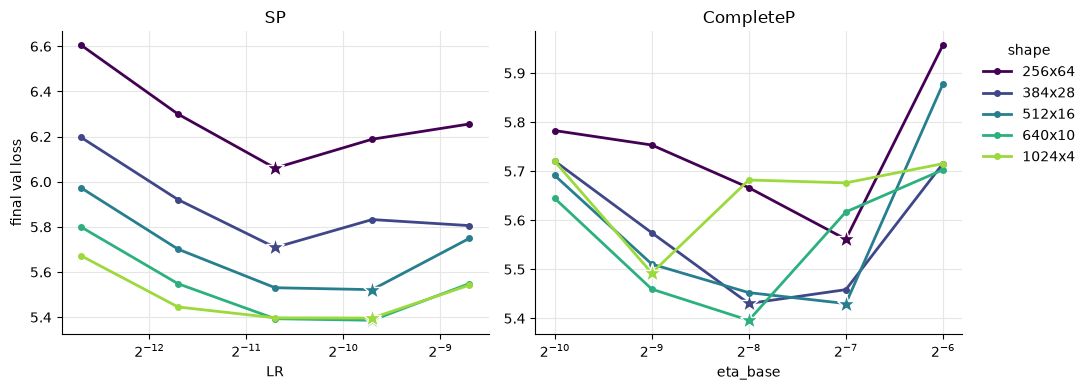
\includegraphics[width=1\linewidth]{figures/tuning_transfer.png}
    \caption{Learning rate sweeps of the tuning runs (10\% of each shape's tokens, compressed schedule). The y-axis is the validation loss at the end of the tuning run, and stars mark the optimum of each shape. Both x-axes are on a $\log_2$ scale.}
    \label{fig:tuning}
\end{figure}

At this tuning horizon, the optimum moves with shape under both parameterisations. For SP it moves down one grid step for the two deepest shapes, and near the optimum the curves are flat: at the three widest shapes, $6\times10^{-4}$ and $1.2\times10^{-3}$ differ by less than 0.01. For CompleteP the optimum does not move steadily with shape: relative to the \sh{512}{16} optimum ($2^{-7}$), it is one grid step lower at \sh{384}{28} and \sh{640}{10} and two grid steps lower at \sh{1024}{4}. At the two widest shapes the transferred $2^{-7}$ is clearly worse than the optimum in the tuning runs (by 0.22 at \sh{640}{10} and 0.18 at \sh{1024}{4}). Measured by the location of the tuning-run optimum, CompleteP therefore shows no better learning rate transfer than SP. Section~\ref{sec:results} shows that the tuning-run optimum can be far from the full-length one (by at least two grid steps for SP at \sh{256}{64}), and the size of this error may depend on shape. The movement of the tuning-run optimum is therefore weak evidence about transfer at full length, and does not contradict the full-run results.

\subsection{Full runs and seed noise}

Every full run uses seed 0 and reads the same tokens in the same order. To estimate run-to-run noise, we trained the base model with two more seeds under each parameterisation. The final losses are $3.387 \pm 0.007$ (SP) and $3.412 \pm 0.008$ (CompleteP), mean $\pm$ standard deviation over 3 seeds. The pooled standard deviation is $\sigma = 0.0076$ with 4 degrees of freedom; its 95\% confidence interval is $[0.005, 0.022]$ (chi-squared interval). Seeds change only the initialisation, not the data order, so $\sigma$ probably understates the full run-to-run variance.

% ============================================================
\section{Results}\label{sec:results}
% ============================================================

\begin{figure*}[t]
    \centering
    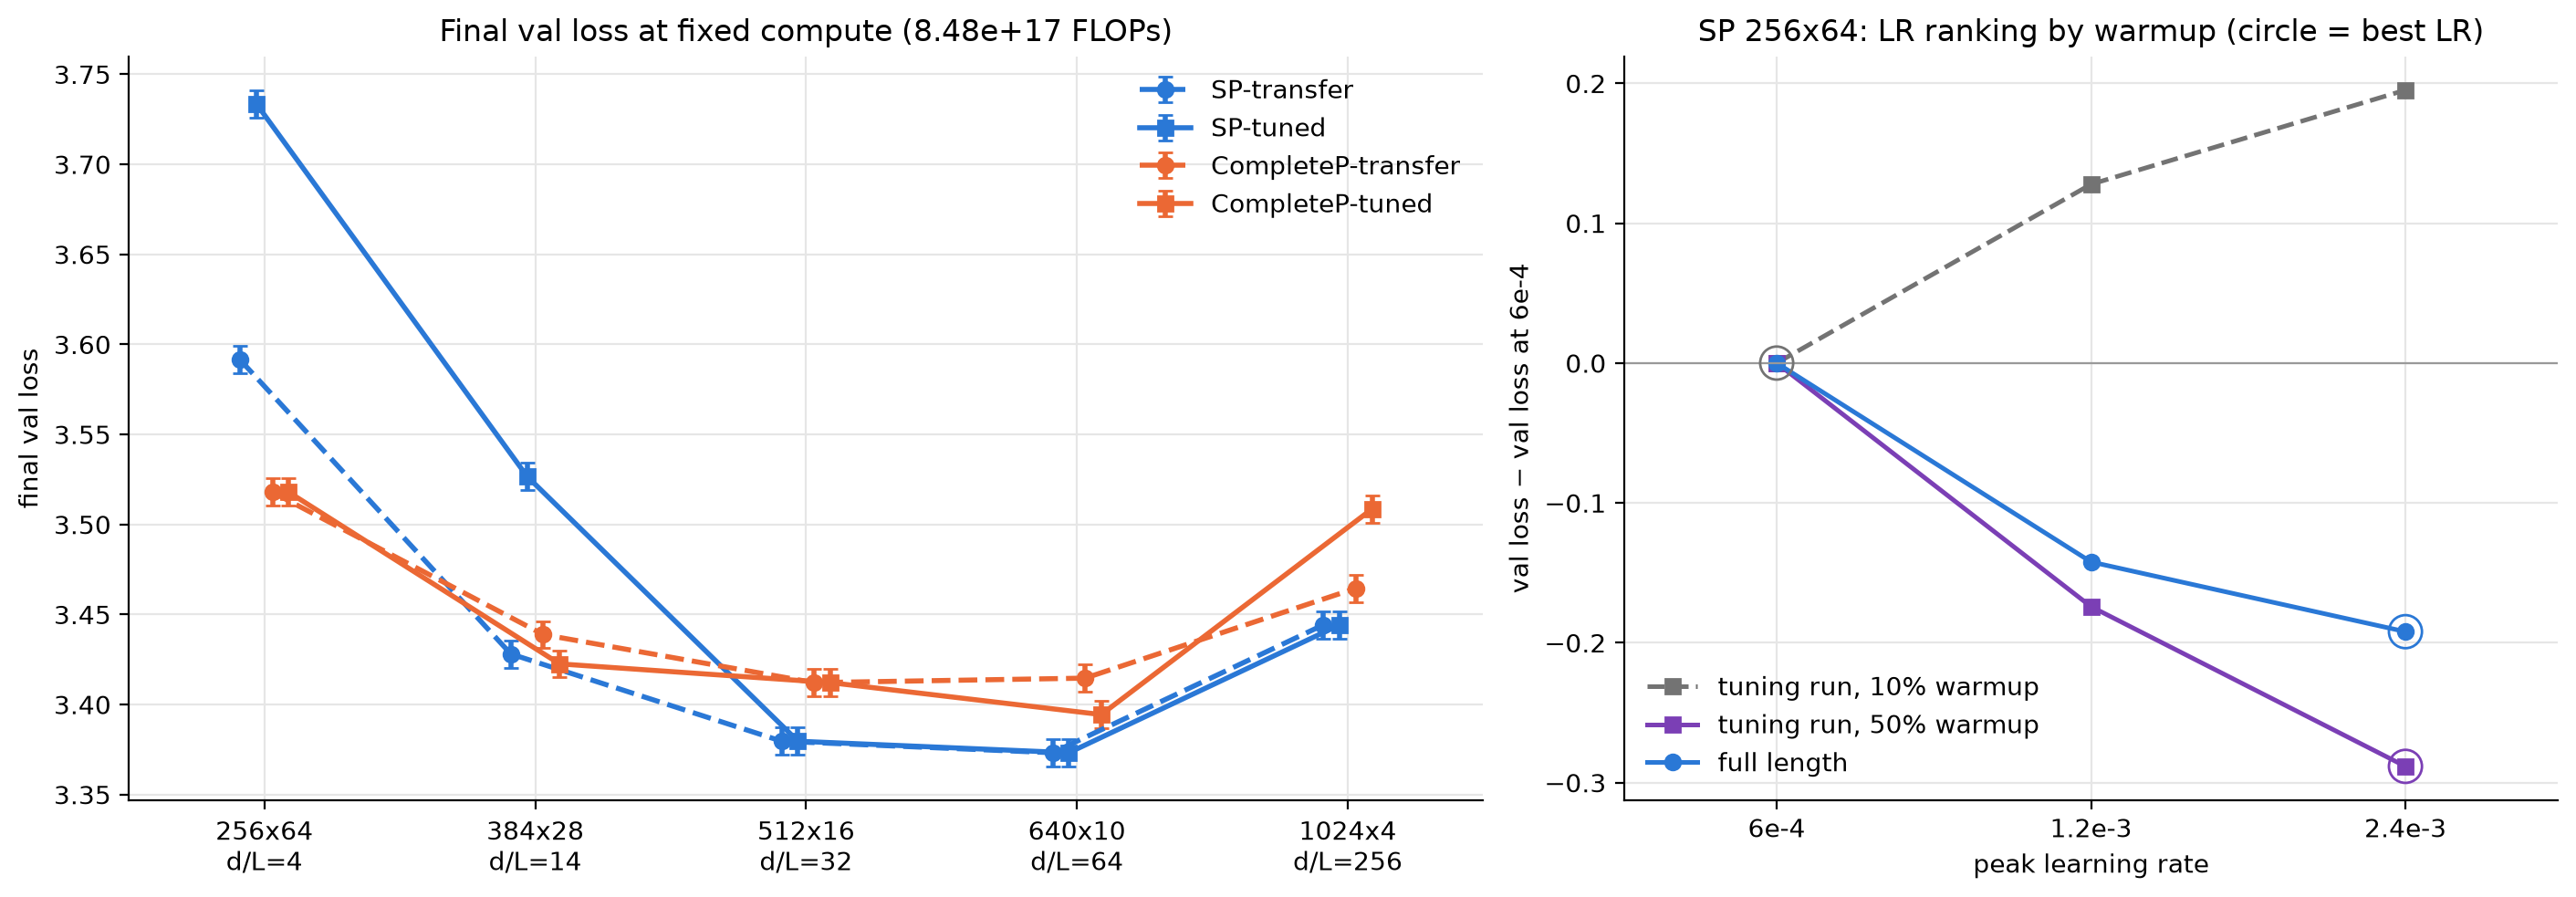
\includegraphics[width=\textwidth]{figures/main_figure.png}
    \caption{\textbf{Left:} final validation loss for each shape at a fixed compute budget of $8.48\times10^{17}$ FLOPs, ordered from deep and narrow to shallow and wide. SP is shown in blue and CompleteP in orange. Dashed lines use the learning rate tuned at \sh{512}{16} and transferred to all shapes; solid lines use a learning rate tuned per shape with short tuning runs (10\% of the tokens). Error bars show $\pm$ the pooled seed standard deviation (0.0076, from 3 seeds per parameterisation at \sh{512}{16}). \textbf{Right:} SP at \sh{256}{64}, validation loss at three peak learning rates, relative to the loss at $6\times10^{-4}$ (negative means better). Circles mark the best learning rate in each setting. Tuning runs with the default 10\% warmup prefer the lowest learning rate. Full-length runs prefer the highest, and so do tuning runs with a 50\% warmup.}
    \label{fig:main}
\end{figure*}

\begin{table}[t]
    \centering
    \small
    \begin{tabular}{lcccc}
        \toprule
        & \multicolumn{2}{c}{SP} & \multicolumn{2}{c}{CompleteP} \\
        \cmidrule(lr){2-3}\cmidrule(lr){4-5}
        Shape & transfer & tuned & transfer & tuned \\
        \midrule
        \sh{256}{64}  & 3.591 & 3.734 & 3.518 & $=$ \\
        \sh{384}{28}  & 3.428 & 3.527 & 3.439 & 3.423 \\
        \sh{512}{16}  & 3.380 & $=$   & 3.412 & $=$ \\
        \sh{640}{10}  & \textbf{3.373} & $=$ & 3.415 & 3.394 \\
        \sh{1024}{4}  & 3.444 & $=$   & 3.465 & 3.509 \\
        \bottomrule
    \end{tabular}
    \caption{Final validation loss of every full run (seed 0). ``$=$'' means the tuned learning rate equals the transferred one, so both conditions share the run to its left. Learning rates are in Table~\ref{tab:tuned_lr}. One extra SP run at \sh{256}{64} with $\eta = 2.4\times10^{-3}$ reaches 3.542.}
    \label{tab:final}
\end{table}

\paragraph{At fixed compute, the best observed width-to-depth ratio is 32 to 64.} Table~\ref{tab:final} and Figure~\ref{fig:main} (left) give the final losses. Under every condition, the deepest shape (\sh{256}{64}, $d/L = 4$) is clearly worst, and the widest (\sh{1024}{4}, $d/L = 256$) is also worse than the middle shapes. The best runs are \sh{512}{16} and \sh{640}{10} ($d/L = 32$ and $64$). We cannot separate these two: under SP they differ by 0.006, less than one seed standard deviation. Too much depth therefore hurts under both parameterisations, with both transferred and tuned learning rates. This agrees with earlier SP studies, and shows that it also holds under CompleteP at this scale.

\paragraph{CompleteP is less sensitive to the transferred learning rate at the deepest shape, but not better in absolute terms.} With the transferred learning rate, the loss rises by 0.212 nats from \sh{512}{16} to \sh{256}{64} under SP, and by 0.106 under CompleteP. The difference between the two gaps combines four single runs, so its standard error is $2\sigma \approx 0.015$, and the difference of 0.106 is about 7 standard errors. Even at the upper end of the confidence interval for $\sigma$, it is still 2.4 standard errors. This assumes that seed noise at \sh{256}{64} is similar to that at \sh{512}{16}, which we have not checked. At the shallower shapes, this also seems to be true though the results are much less significant.

Two observations limit this claim. First, much of the SP gap is due to the transferred learning rate being too low for \sh{256}{64}: at $2.4\times10^{-3}$ the SP gap shrinks to 0.162, and the difference to CompleteP falls to 0.056 (3.7 standard errors, or 1.3 at the upper end of $\sigma$). This best SP value lies on the edge of the learning rates we tried at full length, so the true SP optimum may close the gap further. Second, CompleteP's absolute loss is higher than SP's at \sh{512}{16} (by 0.025 averaged over 3 seeds), \sh{640}{10} and \sh{1024}{4}; its smaller gap is measured from a worse reference. At \sh{256}{64}, CompleteP (3.518) is still better than the best SP run we have (3.542). We conclude that CompleteP makes the deepest shape more robust to an imperfect learning rate, but our data do not show that it reaches a lower loss than a well-tuned SP model.

\paragraph{Tuning on 10\% of the tokens with a compressed schedule picks a learning rate that is too small.} The tuning runs compress the full schedule, so their warmup lasts only 49 to 59 steps, against 489 to 593 in a full run. Their optima can be far from the full-length optimum, and always on the low side in our cases. For SP at \sh{256}{64}, the tuning runs chose $6\times10^{-4}$, but the full run with the transferred $1.2\times10^{-3}$ was 0.14 nats better, and a further full run at $2.4\times10^{-3}$ was better still. This explains why the tuned conditions sometimes underperform the transferred ones in Figure~\ref{fig:main}.

We hypothesise that the short warmup penalises large learning rates early in training, and that the tuning run is too short to recover. To test this, we repeated the SP \sh{256}{64} tuning runs at the three learning rates whose full-length result we know, with the warmup lengthened to 50\% of the steps (278 steps instead of 56; the full run warms up for 557). The ranking of the learning rates reverses and matches the full-length ranking (Figure~\ref{fig:main}, right). The gaps are not proportional, however: the long-warmup tuning run predicts a larger improvement from the highest learning rate than the full run shows, so a long warmup may in turn overestimate the optimum. This test is limited: it covers one shape, one parameterisation and three learning rates with a single seed, and lengthening the warmup also shortens the cosine decay, so the two effects are confounded. Within these limits, our recommendation is to tune on a larger fraction of the data, or at least to keep the warmup from becoming too short in absolute steps.

\begin{figure}[t]
    \centering
    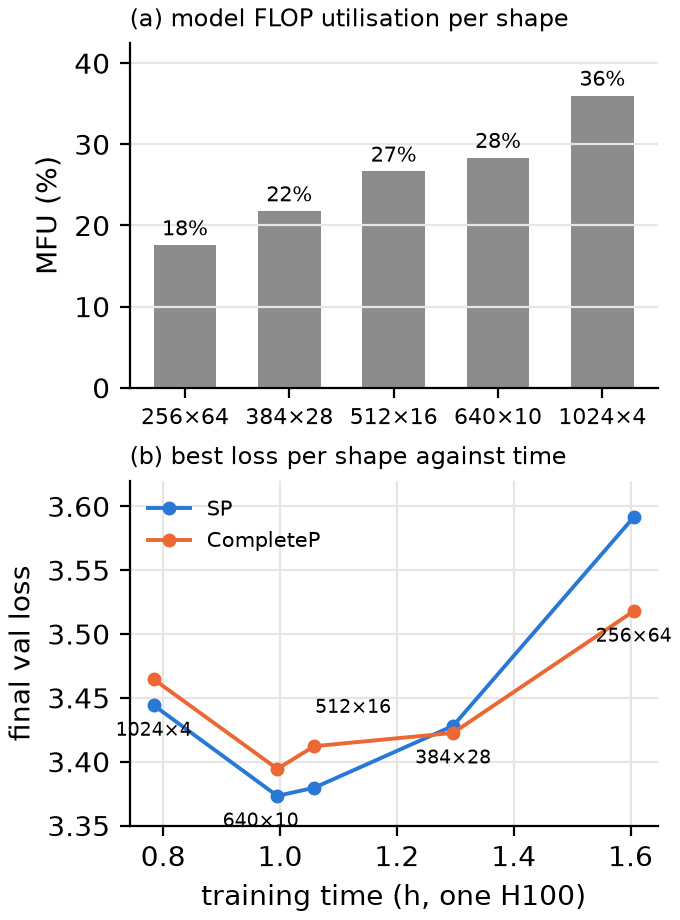
\includegraphics[width=\linewidth]{figures/throughput.png}
    \caption{Training cost of each shape at the same FLOP budget, on one H100 GPU. (a) Model FLOP utilisation (MFU) of each shape, averaged over all its final runs. (b) Best final loss per shape over the transferred and tuned conditions (seed 0), against training time per full run (excluding evaluation, averaged over all final runs of the shape). The extra SP run at \sh{256}{64} with $2.4\times10^{-3}$ (3.542) is not shown.}
    \label{fig:throughput}
\end{figure}

\paragraph{Deep shapes are also slower to train.} All shapes use the same number of FLOPs, but not the same time. A full run of \sh{256}{64} takes 1.61 hours, against 0.78 hours for \sh{1024}{4}, because its MFU is half as high (17.6\% vs 36.0\%, Figure~\ref{fig:throughput}a). At width 256 the matrix multiplications are too small to keep the GPU busy, and each of the 64 layers adds fixed costs such as normalisation, kernel launches and residual additions that the FLOP count ignores. The two deepest shapes also had to use a micro-batch of 16 sequences instead of 32 to fit in memory, with the same tokens per step, which lowers utilisation further. These results are valid for our implementation and setup. Within it, depth costs twice: the deep shapes reach a worse loss \emph{and} take longer to get there (Figure~\ref{fig:throughput}b). \sh{640}{10} is the best choice in both respects, matching \sh{512}{16} in loss while being slightly faster.

% ============================================================
\section{Discussion, limitations and future work}\label{sec:discussion}
% ============================================================

\paragraph{Relation to prior work.} Our results add evidence that too much depth hurts Transformer language models at a fixed compute budget, and that this holds under CompleteP, not only under SP. Consistent with \citet{kaplan2020scaling}, the loss is nearly flat over a range of shapes ($d/L$ from 32 to 64 here), but it rises sharply at the deep end. This fits the view of \citet{levine2020limits} that the useful depth is bounded at a given width. Unlike the final version of \citet{mcleish2025gemstones}, we do not find the deepest models best per FLOP. Our scale is much smaller, however, and embedding parameters make up a large share of our models. Our measurements do confirm their wall-clock argument: at equal FLOPs, the deepest shape takes about twice as long to train as the widest (Figure~\ref{fig:throughput}). Finally, the smaller gap under CompleteP partly supports the motivation of this work, that detuning makes deep models look worse than they are, though it does not account for the whole depth penalty.

\paragraph{Limitations.}
\begin{itemize}[leftmargin=*,itemsep=1pt]
    \item The original question, how much of the depth penalty comes from detuning, remains only partly answered, because our tuning procedure did not find the full-length optima. A full-length sweep at the extreme shapes would resolve this.
    \item Most runs use a single seed, and seed noise is estimated from 3 seeds per parameterisation at the base shape only. The data order is the same in every run.
    \item We test only five aspect ratios, which brackets the optimum but does not locate it precisely.
    \item At 50M non-embedding parameters, embedding parameters and the unembedding are a large share of the parameters and compute, unlike in large production models.
\end{itemize}

\paragraph{Future work.} Two directions are particularly interesting. The first is to revisit our original question with a more reliable tuning procedure, such as longer tuning horizons or full-budget learning rate sweeps. This would give the best achievable loss for each shape and separate the effects of parameterisation and learning rate transfer from those of depth.

The second, motivated by our unexpected tuning results, is to study how the learning rate schedule should be adapted when tuning on a small fraction of the training budget. At our scale, tuning at full length is still feasible, but this becomes prohibitively expensive for larger models. One option is to tune on smaller proxy models and transfer to larger ones, as in $\mu$P \citep{yang2021feature,yang2022tensor} and CompleteP \citep{dey2025completep}. Another is to keep the target model fixed and reduce the number of tokens used for the search.

Work on budgeted training studies how schedules should be adapted to shorter horizons: \citet{li2020budgeted} show that a schedule adapted to the budget beats a longer schedule stopped early, and \citet{chen2022rex} propose alternative schedules for budget-constrained training. Optimising performance at a short horizon is not the same as identifying the learning rate that is best at the full horizon, however. \citet{shleifer2019using} study the transfer of hyperparameters from small proxy datasets to larger ones, but in image classification and without considering schedule compression. Our result also runs against \citet{bjorck2024scaling}, who find that the optimal learning rate decreases as the training horizon grows; short tuning runs should then overestimate the optimum, whereas ours underestimate it. A short warmup is a plausible reason for the reversal. \citet{wortsman2023smallscale} find that a longer warmup makes the loss less sensitive to the learning rate, and \citet{kalra2024warmup} argue that the main benefit of warmup is to let the network tolerate larger learning rates. With only 49 to 59 warmup steps, our tuning runs lose this benefit, which penalises exactly the larger learning rates.

This leaves an open question: \emph{how should the learning rate schedule be adapted during short tuning runs so that the ranking of candidate learning rates best predicts their ranking after full training?} Future work could compare compressed, truncated and modified schedules, including a fixed absolute number of warmup steps, across tuning horizons, model sizes and parameterisations. The objective would be to measure how reliably each strategy identifies the best learning rate for the full budget, rather than the final loss of the short runs.

% ============================================================
\section{Conclusion}
% ============================================================

At the scale studied, excessively deep and narrow Transformers underperform at a fixed compute budget, even under CompleteP. CompleteP makes the deepest shape more robust to a transferred learning rate, but does not reach a lower loss than SP at the best shapes, and our tuning procedure prevented us from reliably quantifying the cost of learning rate detuning. Instead, we found that compressing the learning rate schedule for short tuning runs leaves a very short warmup and systematically underestimates the optimal learning rate. This points to an important direction for future work: compute-efficient tuning procedures that reliably predict the optimal learning rate at the full training horizon.


% ============================================================
% REFERENCES
% ============================================================

\balance
\setlength{\bibsep}{2pt plus 1pt}  % tighter reference list
\bibliographystyle{plainnat}
\bibliography{references}

% ============================================================
% APPENDIX
% ============================================================

\clearpage

\onecolumn
\appendix

\section{Supplementary material}



\subsection{Derivation of the compute budget}\label{app:flops}

We count one multiply and one add as 2 FLOPs. A matrix multiplication of an input of size $m$ by a weight matrix of size $m \times n$ therefore costs $2mn$ FLOPs per token in the forward pass. We count only matrix multiplications. Element-wise operations (LayerNorm, GELU, RoPE, residual additions, softmax) cost $O(Ld)$ or $O(LT)$ per token, which is small next to the $O(Ld^2)$ and $O(LTd)$ terms below.

\paragraph{Non-embedding parameters ($6N$).} Each block has the following weight matrices (no linear layer has a bias):
\begin{itemize}
    \item attention: the query, key and value projections ($3d^2$) and the output projection ($d^2$), i.e.\ $4d^2$, since $n_\text{heads} \cdot d_\text{head} = d$;
    \item MLP: the up projection $d \times 4d$ and the down projection $4d \times d$, i.e.\ $8d^2$.
\end{itemize}
This gives $12d^2$ per block and $N = 12 d^2 L$. We leave out the LayerNorm gains ($2d$ per block plus $d$ for the final LayerNorm), which are not used in a matrix multiplication and are negligible in number. RoPE has no parameters. Each weight is used in exactly one multiply-add per token, so the forward pass costs $2N$ FLOPs per token.

\paragraph{Backward pass (factor 3).} For each matrix multiplication $\vect{y} = W\vect{x}$, the backward pass computes two products of the same size as the forward one: with $\mathcal{L}$ the loss, the gradient with respect to the input, $\frac{\partial \mathcal{L}}{\partial \vect{x}} = W^\top \frac{\partial \mathcal{L}}{\partial \vect{y}}$, which is passed to the previous layer, and the gradient with respect to the weights, $\frac{\partial \mathcal{L}}{\partial W} = \frac{\partial \mathcal{L}}{\partial \vect{y}} \vect{x}^\top$. The backward pass therefore costs twice the forward pass, and a training step costs $3\times$ the forward pass. This turns $2N$ into $6N$, and applies in the same way to the two terms below.

\paragraph{Attention ($6LTd$).} The attention scores and the weighted sum of the values have no parameters, so they are not counted in $N$. For one token at position $t$ and one head, the score $\vect{q}_t^\top \vect{k}_s$ costs $2 d_\text{head}$ FLOPs per key $s$, and adding $a_{ts} \vect{v}_s$ to the output costs another $2 d_\text{head}$. With full (bidirectional) attention over $T$ positions and $n_\text{heads}$ heads, this is $2Td + 2Td = 4Td$ FLOPs per token per layer. Our attention is causal: token $t$ only attends to the $t$ positions up to itself, so on average over a sequence each token attends to about $T/2$ positions, which halves the cost to $2Td$. Over $L$ layers and with the backward pass, this gives $6LTd$. This matches the context term $2LTd$ (forward) of \citet[Eq.~2.2]{kaplan2020scaling}, with $d_\text{attn} = d$. \citet{hoffmann2022training} count the full $T \times T$ matrix for both products, giving $4LTd$ forward and $12LTd$ for training; this is the factor of two mentioned in the main text.

\paragraph{Unembedding ($6dV$).} The final hidden state is multiplied by the $d \times V$ unembedding matrix to give the logits, which costs $2dV$ FLOPs per token forward and $6dV$ for training. With tied embeddings this matrix is also the token embedding, but the input embedding is a table lookup and costs no FLOPs. \citet{hoffmann2022training} count it as a matrix multiplication, which would add another $2dV$ forward. We use the vocabulary padded to $V = 50{,}304$, since this is the matrix size actually computed.

\paragraph{Budget and token counts.} Summing the three terms recovers the formula of the main text, which we write out in terms of $d$ and $L$ using $N = 12d^2L$:
\[
    C_\text{tok} = 6N + 6LTd + 6dV = 72 d^2 L + 6LTd + 6dV .
\]
The budget is set by the base shape \sh{512}{16}: we take 20 tokens per total parameter, $D_\text{base} = 20\,(12 d^2 L + dV) = 20 \times 76.1\text{M} = 1.52$B tokens, and $C = D_\text{base} \cdot C_\text{tok}(512, 16) \approx 8.48 \times 10^{17}$ FLOPs. Every other shape is trained for $D = C / C_\text{tok}(d, L)$ tokens, rounded to a whole number of steps of $128 \times 2048 = 262{,}144$ tokens. Table~\ref{tab:flops} gives the resulting values. At $T = 2048$ the attention and unembedding terms together make up 45\% to 54\% of the compute, which is why we do not drop them as \citeauthor{kaplan2020scaling} do. Their split depends strongly on shape: attention grows with $L$ and the unembedding with $d$, so the deepest and the widest shapes are the ones that a $6N$ count would misestimate the most.

\begin{table}[H]
    \centering
    \small
    \begin{tabular}{lccccccc}
        \toprule
        Shape & $N$ & $dV$ & $6N$ & $6dV$ & $6LTd$ & $C_\text{tok}$ & Tokens $D$ (steps) \\
        \midrule
        \sh{256}{64}  & 50.3M & 12.9M & 302M (52\%) & 77M (13\%)  & 201M (35\%) & 581M & 1.46B (5{,}571) \\
        \sh{384}{28}  & 49.5M & 19.3M & 297M (55\%) & 116M (21\%) & 132M (24\%) & 545M & 1.56B (5{,}932) \\
        \sh{512}{16}  & 50.3M & 25.8M & 302M (54\%) & 155M (28\%) & 101M (18\%) & 557M & 1.52B (5{,}805) \\
        \sh{640}{10}  & 49.2M & 32.2M & 295M (52\%) & 193M (34\%) & 79M (14\%)  & 567M & 1.50B (5{,}707) \\
        \sh{1024}{4}  & 50.3M & 51.5M & 302M (46\%) & 309M (47\%) & 50M (8\%)   & 661M & 1.28B (4{,}890) \\
        \bottomrule
    \end{tabular}
    \caption{Per-token training FLOPs for each shape ($T = 2048$, $V = 50{,}304$), split into the three terms of $C_\text{tok}$ with their share of the total, and the resulting number of training tokens at the fixed budget $C \approx 8.48 \times 10^{17}$ FLOPs.}
    \label{tab:flops}
\end{table}

\subsection{Coordinate check for CompleteP}\label{app:coord}

To check that CompleteP is implemented correctly, we run a coordinate check. We record the mean absolute value of the entries of several activations: the token embedding, the attention and MLP branch outputs, the residual stream after the last block, and the logits. We grow width and depth separately. Under a correct CompleteP these values should stay roughly constant as the model grows, while under SP they are expected to drift. The depth sweep uses the base width ($d = 256$, so $m_d = 1$) and the width sweep uses the base depth ($L = 2$, so $m_L = 1$). The depth sweep therefore tests only the depth part of CompleteP ($\alpha = 1$ residual scaling), and the width sweep tests only the $\mu$P part. The check covers the first 10 training steps only.

\begin{figure}[H]
    \centering
    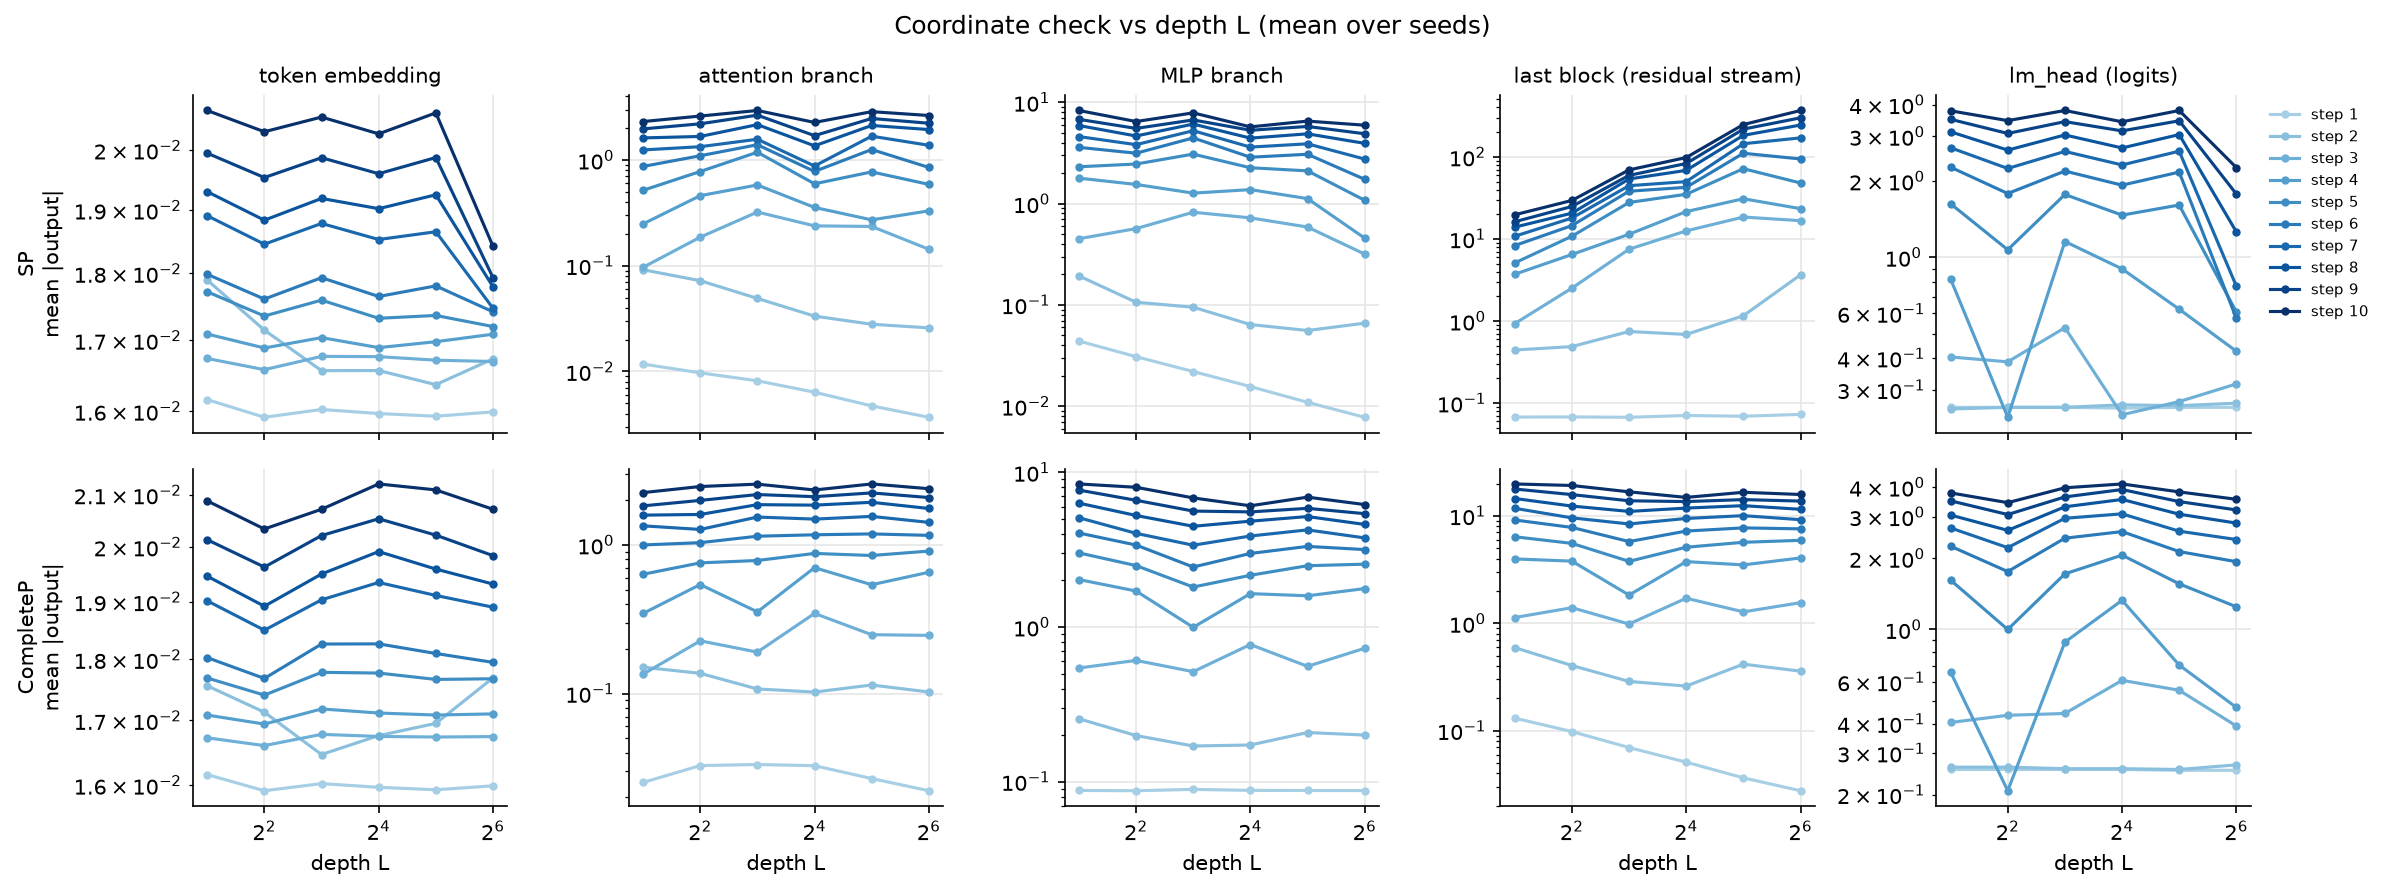
\includegraphics[width=0.6\linewidth]{figures/L_coord_check.png}
    \caption{Coordinate check against depth ($L = 2$ to $64$ at $d = 256$): mean $|\text{output}|$ of each activation at each of 10 training steps (constant learning rate $2^{-8}$, micro-batch 8, mean over 3 seeds; log scale). Attention and MLP values are averaged over all blocks and measured before the residual multiplier. Because of pre-LayerNorm, each branch sees a normalised input, so the SP branch outputs stay roughly flat in depth. The SP residual stream after the last block (before the final LayerNorm) still grows with depth, by about $20\times$ from $L = 2$ to $L = 64$ at step 10, because it sums $L$ unscaled branch outputs. With CompleteP's $L^{-1}$ residual scaling it stays flat.}
    \label{fig:coord_check_depth}
\end{figure}

\begin{figure}[H]
    \centering
    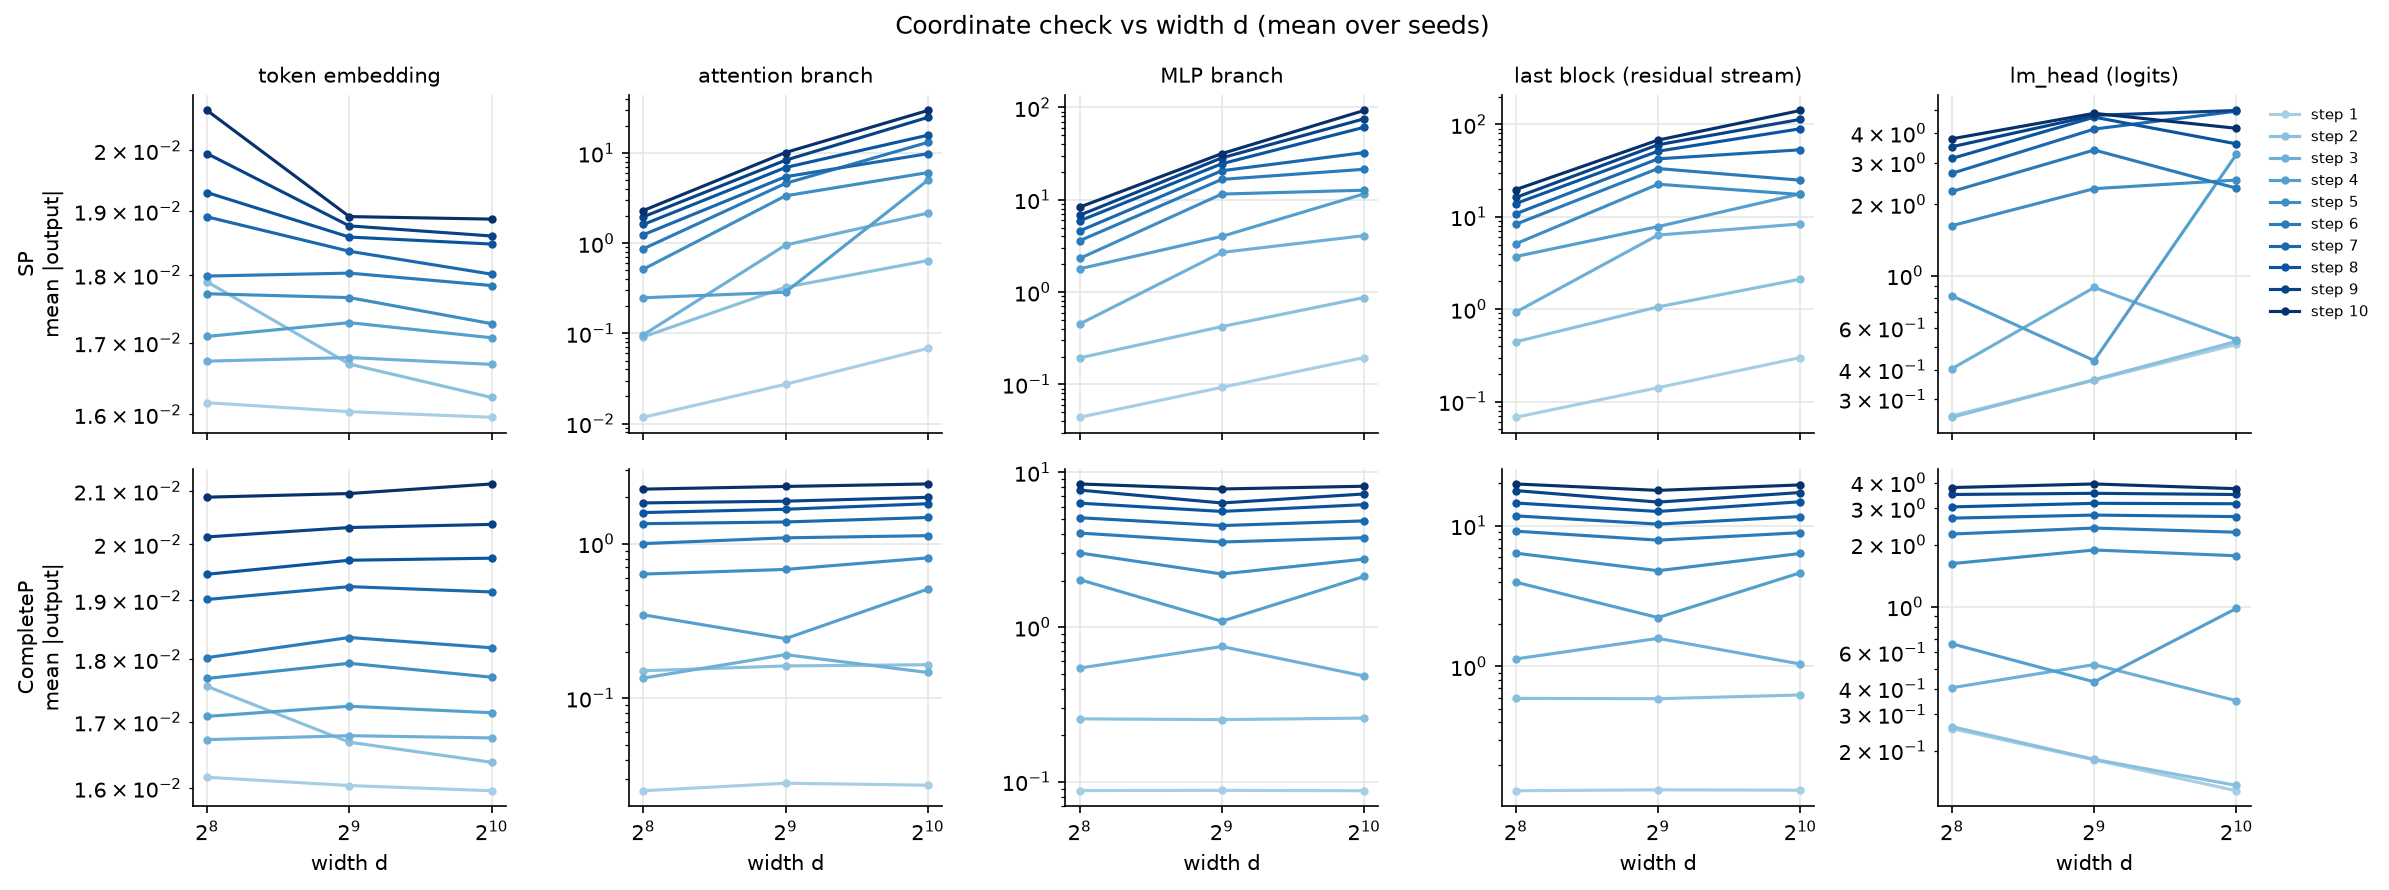
\includegraphics[width=0.6\linewidth]{figures/width_coordinate_check.png}
    \caption{Coordinate check against width ($d = 256$ to $1024$ at $L = 2$), same setup as Figure~\ref{fig:coord_check_depth}. Under SP the attention branch, MLP branch and last-block residual stream grow with width at every step after the first, by roughly $7$ to $13\times$ over a $4\times$ increase in $d$ at step 10. SP uses the same learning rate for every width, so each update of a hidden matrix changes its output by an amount that grows with $d$. CompleteP scales the hidden-matrix learning rate by $m_d^{-1}$, and all its activations stay flat in width; the remaining variation is mostly in the first few steps. The token embedding is nearly flat in both parameterisations. The SP logits vary irregularly with width rather than growing steadily.}
    \label{fig:coord_check_width}
\end{figure}


\end{document}
